\documentclass[a4paper,10pt]{article}
\usepackage[utf8]{inputenc}
\usepackage[brazilian]{babel}
\usepackage{subfig}  %permite o uso do comando subfloat
\usepackage{subcaption}
\usepackage[hmargin=2cm,vmargin=3.5cm,bmargin=2cm]{geometry}
\usepackage{indentfirst}
\usepackage{amsmath}
\usepackage{graphicx}
\usepackage{makeidx}
\usepackage{tocbibind}
 
 \begin{document}	
	\begin{titlepage}
		\begin{center}
		{\large UNIVERSIDADE ESTADUAL DE MARINGÁ}\\[0.2cm]
		{\large CENTRO DE CIÊNCIAS EXATAS}\\[0.2cm]
		{\large DEPARTAMENTO DE FÍSICA}\\[0.2cm]
		{\large LABORATÓRIO DE FÍSICA MODERNA}\\[7.0cm]
		{\bf \huge Velocidade da Luz}\\[7.0cm]
		\end{center}
	{\large Adão Murillo dos Santos \hfill RA:100126}\\[0.7cm]
	{\large João Marcos Fávaro Lopes \hfill RA:98327}\\[0.7cm]
	{\large Lucas Maquedano da Silva \hfill RA:98901}\\[0.7cm]
	{\large Pedro Haerter Pinto \hfill RA:100852}\\[0.7cm]
	{\large TURMA:32 \hfill Professor:Nelson Guilherme Castelli
	Astrath}
	
	\vfill
		\begin{center}
		{\large Maringá,2018}
		\end{center}
	\end{titlepage}

	\tableofcontents
	%\section{Introdução}
Interferência é um fenômeno que ocorre quando duas ou mais ondas sobrepostas se encontram fora de fase, gerando interferências construtivas e destrutivas conforme a interação entre as ondas, sendo a luz uma onda eletro magnética o fenômeno também se aplica a ela, como foi observado no experimento de fenda dupla de Young, as ondas de luz emitidas a partir das fendas se sobrepõem e criam faixas escuras e claras sendo estas os mínimos e máximos de intensidade luminosa gerados pela interferência. Michelson montou o seu interferômetro, aparato que foi utilizado no experimento contido neste relatório, a fim de mostrar a influência do "éter luminoso"(suposto meio necessário para a propagação da luz) sobre a velocidade da luz, o experimento mostrou a não existência do éter. 
No presente relatório, o interferômetro de Michelson será utilizado para determinar o comprimento de onda de um lazer.

	%\section{Desenvolvimento Teórico}
\subsection{Velocidade da Luz}
O feixe de luz que sai do laser é refletido em um ângulo $\theta$ com a reta normal do espelho rotatório ($MR$), como mostrado na $Figura 1$, em direção ao ponto $S$ do espelho fixo ($MF$). Ao passo que o espelho $MR$ rotaciona, sua reta normal irá variar em ângulo  $\Delta \theta$, resultando em um novo ângulo de incidência $\theta1$. O feixe incidirá então no ponto $S1$ do espelho $MF$.
\begin{figure}[!ht]
	\centering
	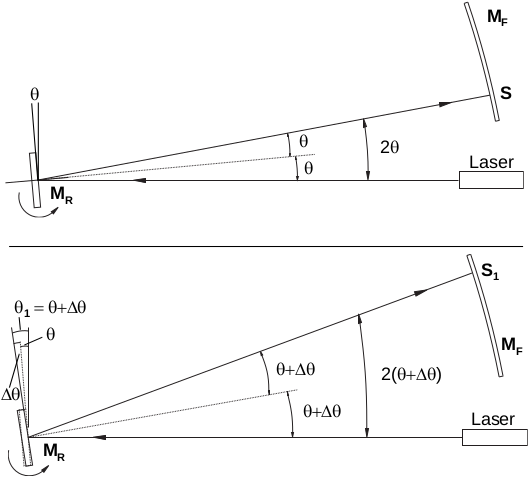
\includegraphics[scale=0.4]{2.png}
	\caption{Diagrama do caminho óptico percorrido pelo feixe e detalhe da diferença angular decorrente da rotação do espelho $MR$}
\end{figure} 
Sendo $D$ a distância entre os espelhos, a diferença de caminho entre os feixes é dada por:

\begin{equation}
	S1-S = D(2\theta1 - 2\theta)=D[2(\theta+\Delta\theta)-2\theta]= 2D\Delta		\theta
\end{equation}
Uma análise semelhante pode ser empregada na seguinte montagem:

\begin{figure}[!ht]
	\centering
	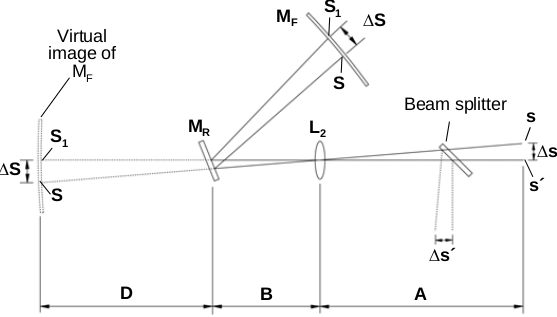
\includegraphics[scale=0.4]{3.png}
	\caption{Diagrama do caminho óptico semelhante ao arranjo experimental \cite{PASCO}}
\end{figure}
Onde o deslocamento do ponto imagem ($\Delta S'$) decorrente da rotação do espelho $MR$ é igual ao deslocamento $\Delta S$ da imagem virtual no espelho $MF$, a qual é determinada pela relação:

\begin{equation}
	\Delta S'= \Delta S=(-i/o)\Delta S
\end{equation}
Em que $i$ é a distância da imagem até a lente e $o$ a distância do objeto até a mesma ($L2$). Pela $Figura2$ obtem-se que:

\begin{equation}
	(-i/o)\Delta S=\frac{A}{D+B}\Delta S
\end{equation}
 
Substituindo o valor de $\Delta S$ obtido na eq. $1$:

\begin{equation}
	\Delta S'=\frac{2DA\Delta\theta}{D+B}
\end{equation}

Sabendo-se que o ângulo $\Delta\theta$ depende da velocidade de rotação ($\omega$) do espelho $MR$, do trajeto do feixe entre os espelhos ($2D$) e da velocidade $c$ da luz, resulta:

\begin{equation}
	\Delta\theta=\frac{2D\omega}{c}
\end{equation}

Com a igualdade da eq. $4$

\begin{equation}
	\Delta S'=\frac{4D^{2}A\omega}{c(D+B)}
\end{equation}

Isolando-se $c$:

\begin{equation}
	c=\frac{4D^{2}A\omega}{(D+B)\Delta S'}
\end{equation}
substituindo $\omega$ por $2\pi f$
\begin{equation}
	c=\frac{8D^{2}A\pi f}{(D+B)\Delta S'}
\label{eq:C}
\end{equation}
Variando então os parâmetros $\omega$ e, consequentemente, $\Delta S'$ e conhecendo os demais valores das constantes, é posível calcular a velocidade $c$ da luz.

\subsection{Desvios}
\subsubsection{Desvio de Medidas Diretas}
Para este experimento, tem-se como medidas diretas, as distâncias entre os espelhos e lentes, e a variação da posição do feixe de luz no microscópio. Para as medidas de distancia foi utilizada uma trena com o erro associado de $0,005m$ e para o $\Delta s$ tem-se o erro de $2,5mm$,pois a menor variação que é possível medir é de $5mm$.
\subsubsection{Desvio de Medidas Indiretas}
Para o cálculo de Velocidade da luz é utilizada a equação \ref{eq:C} e para o cálculo dos erros, é aplicado o logaritmo neperiano em ambos os lados da equação, tornando-se:

\begin{equation}
	ln(c)=ln(\frac{8D^{2}A\pi f}{(D+B)\Delta S'})
\end{equation}

e utilizando propriedades de logaritmos, é obtido

\begin{equation}
	ln(c)=ln(8D^{2}A\pi f)-ln((D+B)\Delta S')
\end{equation}
\begin{equation}
	ln(c)=ln(8A) + 2ln(D) - [ln(D+B)+ln(\Delta S)]
\end{equation}
diferenciando a equação
\begin{equation}
	\frac{dc}{c}=\frac{dA}{8A} + \frac{2dD}{d} + \frac{dA}{A+B} + \frac{dB}{A+B}+\frac{d\Delta S}{\Delta S}
\end{equation}
e fazendo $d\rightarrow \delta$ para poder ser aplicado os erros medidos experimentalmente. Onde $\delta$ representa o erro associado.
\begin{equation}
	\frac{\delta c}{c}=\frac{\delta A}{8A} + \frac{2\delta D}{d} + \frac{\delta A}{A+B} + \frac{\delta B}{A+B}+\frac{\delta \Delta S}{\Delta S}
\label{eq:err}
\end{equation}

	\section{Desenvolvimento Experimental}
\subsection{Materiais e Métodos}
Foram utilizados para a realização do experimento:
\begin{itemize}
	\item Tubo e/m;
	\item Duas bobinas de Helmholtz com 15 cm de raio;
	\item Régua espelhada;
	\item Duas fontes DC;
	\item Multímetros;
	\item Cabos de energia.
\end{itemize}

O experimento consiste em um tubo com gás rarefeito  ao qual é acoplado um filamento de metal. Liga-se o filamento a uma fonte em uma tensão menor que 6,0 $volts$, então ao passar uma corrente pelo fio este emitirá elétrons os quais serão defletidos em forma de feixe, que ionizarão o gás formando um rastro de luz. Em seguida, deve-se regular o foco do feixe através do botão a frente do equipamento. É submetido o tubo a um campo margnético uniforme por meio de uma bobina cuja corrente e voltagem podem ser controladas pelo painel frontal. O campo defletirá o fixe de elétrons em um círculo que poderá ser medido por uma régua ao fundo do tubo. Para se calcular a razão carga-massa é preciso variar a voltagem da bobina e consequentemente o raio ao qual o feixe é defletido. A variação é dada entre 150 e 300 $volts$ atingidas de 10 em 10 $volts$.

\subsection{Dados Obtidos Experimentalmente}
Após a realização do experimento duas vezes, foram obtidos os dados e utilizando os mesmos, foi gerado em programa o gráfico da Figura \ref{fig},contendo a diferença de potencial aplicada (DDP) com o respectivo raio do feixe de elétrons ($r$), e calculando o ajuste linear obteve-se a equação $V = 98079.57r^2 $

\begin{figure}[!ht]
	\centering
		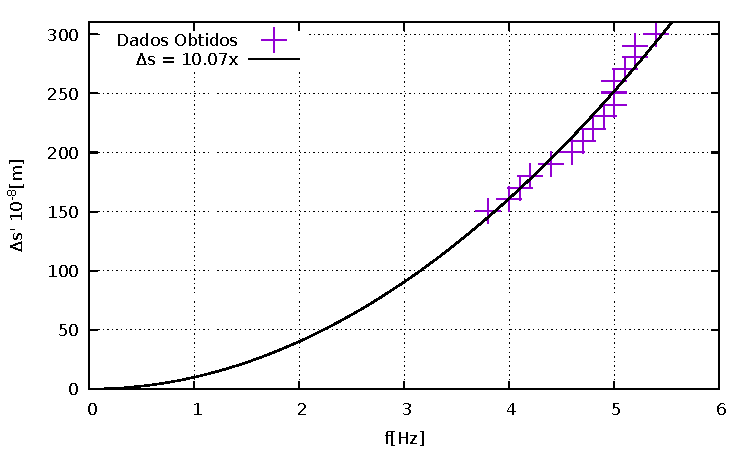
\includegraphics[scale= 1.0]{graf/e_m.pdf}
	\caption{Relação entre a diferença de potencial($DDP$) usado para acelerar os elétrons e o raio ($r$) formado pelos elétrons, com equação igual a $V = (98079.57\pm 1219.33)r^2$}
\label{fig}
\end{figure}

\subsection{Interpretação dos Resultados}

Sabendo-se que
\begin{equation}
	\frac{e}{m}=\frac{2V\left(\frac{5}{4}\right)^3a^2}{[N\mu _0 Ir]^2}
\end{equation}
é possível fazer
\begin{equation}
	V = \frac{[N \mu _0 I]^2\left(\frac{e}{m}\right)}{2(5/4)^3a^2}r^2
\end{equation}
onde fazendo
\begin{equation}
\begin{split}
	\lambda = \frac{[N \mu _0 I]^2\left(\frac{e}{m}\right)}{2(5/4)^3a^2}\\
	V = \lambda r^2
\label{eq1}
\end{split}
\end{equation}
sabendo que
\begin{equation}
	V = 98079,57r^2
\label{eq2}
\end{equation}
igualando \ref{eq1} e \ref{eq2} é obtido
\begin{equation*}
	\lambda = 98079,57
\end{equation*}
e portanto
\begin{equation}
	98079,57 =  \frac{[N \mu _0 I]^2\left(\frac{e}{m}\right)}{2(5/4)^3a^2}
\end{equation}
onde $N,\mu _0,I$ e $a$ são:
\begin{equation*}
	\begin{split}
		N=130\\
		\mu _0 =4\pi\times10^{-7}\\
		I=(1,24\pm0,01)A\\
		a=0,15cm
	\end{split}
\end{equation*}
substituindo os valores
\begin{equation}
	98079,57 =  \frac{[130*4\pi\times10^{-7}*1,24]^2\left(\frac{e}{m}\right)}{2(5/4)^30,15^2}
\end{equation}
e portanto
\begin{equation}
	\frac{e}{m}=\frac{98079,57*2*(5/4)^3*0,15^2}{[130*4\pi\times10^{-7}*124]^2}
\end{equation}
resolvendo
\begin{equation}
	\frac{e}{m}=(2,10\pm0,08)\times10^{11}Q/kg
\end{equation}
Comparando com o valor de 
\begin{equation}
	c=1,76\times10^{} Q/Kg
\end{equation}        
obtido na literatura \cite{PASCO}, resulta em um erro relativo ($Er$) de:
\begin{equation}
	Er=\left|\frac{1,76\times10^{11}-2,10\times10^{11}}{1,76\times10^{11}}\right|*100\%= 19,31\%
\end{equation}

Estes erros estão associados a obtenção dos dados, sendo
possível um erro de paralaxe durante a visualização dos dados na régua espelhada, o que acarreta uma variação do valor de $c$ predito na literatura. Porém, mesmo com todos os fatores associados, o erro  de
19,31\% é aceitável dentro da precisão necessária para a realização do experimento.


	%\section{Conclusão}
Podemos dizer, com base no desvio obtido, que o experimento realizado foi bem sucedido. Mesmo com um erro pequeno, pode-se salientar alguns motivos pelo mesmo, como o movimento de pessoas no laboratório e a vibração do ar condicionado, visto que o aparelho é muito sensível, também, possíveis erros humanos na hora da contagem de franjas. Por fim, com o êxito do experimento, conseguimos determinar o índice de refração do ar satisfatoriamente. 

	
\vspace{3cm}
	\begin{thebibliography}{1}
    	\bibitem{PASCO}PASCO, \it{Speed of Light Apparatus}, Instruction Manual and 	Experiment Guide for the PASCO Scientific Model OS-9261A, 62 and 63A.
	\end{thebibliography}	
	
\end{document}

